
The actual proof of Theorem~\ref{thm:amt-comp-reduc-em-coh} is slightly stronger than its statement
as it creates a degree~$\dbf$ bounding~$\emo$ together with a computable instance~$X$ of~$\amt$
such that $\dbf$ bounds no solution to~$X$. Therefore, having solutions to multiple tournaments in parallel
is not enough to compute a solution to~$X$.
One may however ask whether \emph{sequential} applications of~$\emo$
(that is, defining a tournament such that every transitive subtournament will be used to define another tournament
and so on) is enough to compute a solution to~$X$.

Answering negatively this question requires to diagonalize against solutions $Y_0$ to computable instances of~$\emo$,
but also against solutions $Y_1$ to $Y_0$-computable instances of~$\emo$ and so on. The difficulty comes
from the fact that diagonalizations happen at finite stages, at which we have only access to a finite approximation
of~$Y_0$, and so to a finite part of the $Y_0$-computable instances of~$\emo$.
Thankfully, we only need a finite piece of an $\emo$-instance to diagonalize against its solutions.

In this section, we develop a framework for building an $\omega$-structure~$\Mcal$ satisfing some principle $\Psf$
such that every function in $\Mcal$ is dominated by a single $\emptyset'$-computable function.
Since by definition, the first-order part of an $\omega$-structure is the set of standard natural numbers,
$\omega$-structures are characterized by their second-order part. An $\omega$-structure
satisfies $\rca$ if and only if its second-order part is a Turing ideal, i.e.,
a set of reals $\Ical$ closed under the effective join and the Turing reduction.

The whole construction will be done by iterating uniformly and $\emptyset'$-effectively
the forcing constructions presented in the previous sections.
We will not directly deal with the concrete forcing notion used for constructing solutions
to $\emo$-instances. Instead, we will manipulate an abstract partial order of forcing conditions.
Abstracting the construction has several advantages:
\begin{itemize}
	\item[1.] It enables the reader to focus on the operations which are the essence of the construction.
	The reader will not be distracted by the implementation subtleties of $\emo$ which are not insightful 
	to understand the overall structure.
	\item[2.] The construction is more modular. We will be able to implement modules for~$\emo$
	and~$\wkl$ independently, and combine them in section~\ref{sect:separating-amt-combined} 
	to obtain a proof that~$\emo \wedge \allowbreak \wkl$ does not imply~$\amt$, 
	and this without changing the main construction.
	This also enable reverse mathematicians to prove that other principles do not imply~$\amt$ without having to reprove
	the administrative aspects of the construction.
\end{itemize}

We shall illustrate our definitions with the case of~$\coh$ in order to give a better
intuition about the abstract operators we will define. As explained in section~\ref{sect:emo-computable-reducibility}, 
the separation of~$\coh$ from~$\amt$
is already a consequence of the separation of~$\emo$ from~$\amt$. Therefore implementing the framework
with~$\coh$ is only for illustration purposes.

\subsection{Support}

The first step consists of defining the abstract partial order which will represent the partial
order of forcing conditions. We start with an analysis of the common aspects of the different
forcing notions encountered until yet, in order to extract their essence and define the abstract operators.
In the following, we shall employ \emph{stage} to denote a temporal step in the construction.
An \emph{iteration} is a spatial step representing progress in the construction of the Turing ideal.
Multiple iterations are handled at a single stage. 
\smallskip

\emph{Parts of a condition}. When constructing cohesive sets for~$\coh$
or transitive subtournaments for~$\emo$, we have been working in both cases with \emph{conditions}
representing parallel Mathias conditions. We shall therefore associate to our abstract notion of condition
a notion of~\emph{part} representing one of the solutions we are building.
A single abstract condition will have multiple \emph{parts} representing the various candidate
solutions constructed in parallel for the same instance.

For example, in the forcing notion for~$\coh$, a condition~$c = (F_\nu : \nu \in 2^n)$
can be seen as $2^n$ parallel Mathias conditions $(F_\nu, R_\nu)$ where $R_0, R_1, \dots$
is the universal instance of $\coh$. In this setting, the parts of~$c$ are the pairs $\tuple{c, \nu}$ for each~$\nu \in 2^n$.
One may be tempted to get rid of the notion of condition and directly deal with its parts
since in $\coh$, a condition is only the tuple of its parts.
However, in the forcing notion $c = (\vec{F}, \Ccal)$ for~$\emo$, the parts are interdependent
since adding element to some~$F_\nu$ will remove inconsistent covers from~$\Ccal$
and therefore may restrict the reservoirs of the other parts.
\smallskip

\emph{Satisfaction}. As explained, a part represents the construction of one solution, whereas a condition
denotes multiple solutions in parallel. We can formalize this intuition by defining
a \emph{satisfaction function} which, given a part of a condition, returns the collection of the sets
satisfying it. For example, a set~$G$ satisfies part~$\nu$ of the $\coh$ condition~$c = (F_\nu : \nu \in 2^n)$
if it satisfies the Mathias condition $(F_\nu, R_\nu \setminus [0, max(F)])$,
in other words, if $F_\nu \subseteq G$ and $G \setminus F_\nu \subseteq R_\nu \setminus [0, max(F_\nu)]$.
\smallskip


\begin{figure}[htbp]
\begin{center}
\scalebox{0.9}{
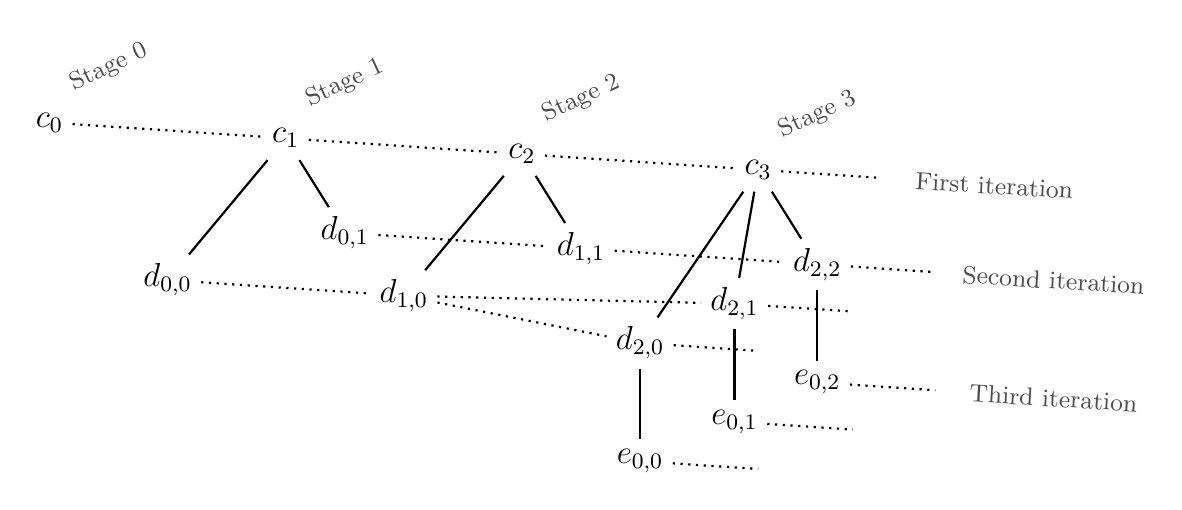
\begin{tikzpicture}[x=1.5cm, y=1cm, thick,
		node/.style={inner sep=3pt, minimum size=1.5em, font=\large{#1}},
		stage/.style={node,rotate=25,opacity=0.7},
		label/.style={node,rotate=-3.5,opacity=0.7}
]

  \node[node] (c0) at (0, 10) {$c_0$};
	\node[node] (c1) at (2, 9.8) {$c_1$};
	\node[node] (c2) at (4, 9.6) {$c_2$};
	\node[node] (c3) at (6, 9.4) {$c_3$};
	
	\node[node] (d00) at (1, 8) {$d_{0,0}$};
	\node[node] (d01) at (2.5, 8.6) {$d_{0,1}$};
	\node[node] (d10) at (3, 7.8) {$d_{1,0}$};
	\node[node] (d11) at (4.5, 8.4) {$d_{1,1}$};
	\node[node] (d20) at (5, 7.2) {$d_{2,0}$};
	\node[node] (d21) at (5.8, 7.7) {$d_{2,1}$};
	\node[node] (d22) at (6.5, 8.2) {$d_{2,2}$};

	\node[node] (e00) at (5, 5.7) {$e_{0,0}$};
	\node[node] (e01) at (5.8, 6.2) {$e_{0,1}$};
	\node[node] (e02) at (6.5, 6.7) {$e_{0,2}$};

	\node[label] (t1) at (8, 9.2) {\small First iteration};
	\node[label] (t2) at (8.5, 8) {\small Second iteration};
	\node[label] (t3) at (8.5, 6.5) {\small Third iteration};

	\node[stage] (l1) at (0.5,10.7) {\small Stage 0};
	\node[stage] (l2) at (2.5,10.5) {\small Stage 1};
	\node[stage] (l3) at (4.5,10.3) {\small Stage 2};
	\node[stage] (l4) at (6.5,10.1) {\small Stage 3};
	
	\draw[dotted] (c0) -- (c1) -- (c2) -- (c3) -- (7,9.3);


	% Stage 1
	\draw (c1) -- (d00);
	\draw (c1) -- (d01);

	% Stage 2
	\draw (c2) -- (d10);
	\draw (c2) -- (d11);
	\draw[dotted] (d00) -- (d10);
	\draw[dotted] (d01) -- (d11);

	% Stage 3
	\draw (c3) -- (d20);
	\draw (c3) -- (d21);
	\draw (c3) -- (d22);
	\draw[dotted] (d10) -- (d20);
	\draw[dotted] (d10) -- (d21);
	\draw[dotted] (d11) -- (d22);

	% Stage 4
	\draw (d20) -- (e00);
	\draw (d21) -- (e01);
	\draw (d22) -- (e02);

	% Extension
	\draw[dotted] (d22) -- (7.5, 8.1);
	\draw[dotted] (d21) -- (6.8, 7.6);
	\draw[dotted] (d20) -- (6, 7.1);
	\draw[dotted] (e00) -- (6,5.6);
	\draw[dotted] (e01) -- (6.8, 6.1);
	\draw[dotted] (e02) -- (7.5, 6.6);

\end{tikzpicture}
}
\end{center}
\caption{Example of construction of a Turing ideal by an iterative forcing
	in which conditions may have multiple parts. The nodes are the conditions,
	the dotted edges are condition extensions and the plain
	edges are the parts of the conditions.} 
\end{figure}



\emph{Initial condition}. 
In a standard (i.e.\ non-iterative) forcing, we build an infinite decreasing sequence
of conditions, starting from one initial condition~$c_0$. In $\coh$, this initial condition is~$(\emptyset, \varepsilon)$,
where~$\varepsilon$ is the empty string. Since~$R_\varepsilon = \omega$, this coincides with the standard
initial Mathias condition~$(\emptyset, \omega)$.
In an iterative forcing, we add progressively new iterations by starting a new decreasing sequence of conditions
below each part of the parent condition. Since $\coh$ admits a universal instance, there is no need to choose
which instance we want to solve at each iteration. However, in the case of~$\emo$, we will take a new $\emo$-instance
each time, so that the resulting Turing ideal is the second-order part of an $\omega$-model satisfying $\emo$.
Therefore, an $\emo$-condition is in fact a condition~$(\vec{F}, \Ccal, R)$ where $R$ is an instance of~$\emo$.
The chosen instance of~$\emo$ will be decided at the initialization of a new iteration and will be preserved
by condition extension. The choice of the instance depends only on the iteration level. Therefore we can
define an initialization function which, given some integer, returns the initial condition together with the chosen instance.
\smallskip

\emph{Parameters}.
The difficulty of the iterative forcing comes from the fact that an instance of the principle~$\Psf$
may depend on the previous iterations. During the construction, the partial approximations
of the previous iterations become more and more precise, enabling the instance at the next iteration to be
defined on a larger domain. In the definition of our abstract partial order, we will use a formal parameter $D$
which will represent the join of the constructed solutions in the previous iterations.
For example, in the formal definition of the partial order for~$\coh$, we will say that
some condition $d = (E_\mu : \mu \in 2^m)$ extends another condition $c = (F_\nu : \nu \in 2^n)$ if~$m \geq n$,
and $(E_\mu, R^D_\mu \setminus [0, max(E_\mu)])$ 
Mathias extends $(F_\nu, R^D_\nu \setminus [0,max(F_\nu)])$ for each~$\nu \preceq \mu$. 
This syntactic constraints has to be understood as $(E_\mu, R^X_\mu \setminus [0, max(E_\mu)])$ 
Mathias extends $(F_\nu, R^X_\nu \setminus [0,max(F_\nu)])$
for every set $X = X_0 \oplus \dots \oplus X_{n-1}$ such that~$X_i$ satisfies the ancestor of~$d$ in the iteration axis
at the $i$th level. In the case of $\coh$, only a finite initial segment of $X$ is needed to witness
the extension.

We are now ready to define the notion of module support. 

\begin{definition}[Module support]
A \emph{Module support} is a tuple~$\tuple{\Pb, \Ub, \parop, \iniop, \satop}$ where
\begin{itemize}
	\item[(1)] $(\Pb, \leq_\Pb)$ is a partial order. The set~$\Pb$ has to be thought of as the set of forcing conditions.
	Therefore, the elements of~$\Pb$ will be called \emph{conditions}.
	\item[(2)] $\Ub$ is a set of \emph{parts}. 
	The notion of part is due to the fact that most of our forcing conditions represent multiple
	objects built in parallel.
	\item[(3)] $\parop : \Pb \to \Pcal_{fin}(\Ub)$ is a computable function which, given some condition~$c \in \Pb$,
	gives the finite set of parts associated to~$c$.
	\item[(4)] $\iniop : \Nb \to \Pb$ is a computable function which, given some integer $n$ representing
	the iteration level, provides the initial condition of the forcing at the $n$th iteration.
	\item[(5)] $\satop : \Ub \to \Pcal(2^\omega)$ is a function which, given some part~$\nu$ of some condition~$c$,
	returns the collections of sets satisfying it.
\end{itemize}
Furthermore, a module support is required to satisfy the following property:
\begin{itemize}
	\item[(a)] If~$d \leq_\Pb c$ for some~$c, d \in \Pb$, then there is a function~$f : \parop(d) \to \parop(c)$
such that $\satop(\nu) \subseteq \satop(f(\nu))$ for each~$\nu \in \parop(d)$. We may write it $d \leq_f c$
	and say that $f$ is the \emph{refinement function witnessing $d \leq_\Pb c$}.
\end{itemize}
\end{definition}

Given two conditions~$c, d \in \Pb$ such that~$d \leq_f c$, 
we say that $f$ \emph{forks} part~$\nu$ of $c$ if $|f^{-1}(\nu)| \geq 2$. 
This forking notion will be useful in the definition of a module.
Let us illustrate the notion of module support by defining one for~$\coh$.
\smallskip

\emph{Module support for~$\coh$}.
Define the tuple  $\tuple{\Pb, \Ub, \parop, \iniop, \satop}$ as follows:
$\Pb$ is the collection of all conditions~$(F_\nu : \nu \in 2^n)$ where~$F_\nu$ is a finite set of integers.
Given some~$d = (E_\mu : \mu \in 2^m)$ and $c = (F_\nu : \nu \in 2^n)$, $d \leq_\Pb c$ if~$m \geq n$,
and $(E_\mu, R^D_\mu \setminus [0, max(E_\mu)])$ Mathias extends 
$(F_\nu, R^D_\nu \setminus [0, max(F_\nu)])$ for each~$\nu \preceq \mu$.
Let~$\Ub$ be the set of all pairs $\tuple{(F_\nu : \nu \in 2^n), \nu}$ where~$\nu \in 2^n$.
Given some condition~$c = (F_\nu : \nu \in 2^n) \in \Pb$, $\parop(c) = \{\tuple{c, \nu} : \nu \in 2^n\}$.
For every level~$n \geq 0$, $\iniop(n) = (\emptyset, \varepsilon)$.
Define $\satop(\tuple{(F_\nu : \nu \in 2^n), \nu})$ to be the collection of all sets satisfying the Mathias condition
$(F_\nu, R_\nu \setminus [0, max(F_\nu)])$.

We now check that property (a) holds.
Let~$d = (E_\mu : \mu \in 2^m)$ and $c = (F_\nu : \nu \in 2^n)$ be such that $d \leq_\Pb c$. In particular, $m \geq n$.
Define~$f : \Ub \to \Ub$ by $f(\tuple{d, \mu}) = \tuple{c, \mu \uh n}$. 
We claim that~$f$ is a refinement function witnessing~$d \leq_\Pb c$.
$\satop(\tuple{d,\mu})$ is the collection of sets satisfying the Mathias condition 
$\tilde{d} = (E_\mu, R_\mu \setminus [0, max(E_\mu)))$
and $\satop(\tuple{c, \mu \uh n})$ is the collection of sets 
satisfying $\tilde{c} = (F_{\mu \uh n}, R_{\mu \uh n} \setminus [0, max(F_{\mu \uh n})))$.
Since $\mu \uh n \preceq \mu$, $\tilde{d}$ Mathias extends $\tilde{c}$ by definition of~$\satop$.
Considering the Mathias conditions, every set satisfying $\tilde{d}$ satisfies $\tilde{c}$,
so $\satop(\tuple{d,\mu}) \subseteq \satop(f(\tuple{d,\mu}))$. Therefore the property (a) of a module support is satisfied.

\subsection{Modules}

We previously defined the abstract structure we shall use as a support of the construction.
The next step consists of enriching this structure with a few more operators which will enable us to decide $\Sigma^0_1$ properties
over the constructed sets. The success or failure in forcing some property will depend on the parts of a condition. Note that at a finite stage, we handle a finite tree of conditions. We can therefore cover all cases by asking finitely many questions.
Let us go back to the $\coh$ example, and more precisely how we decided $\Sigma^0_1$ properties over it.

\emph{Iteration 1}. At the first iteration, we would like to decide whether
the $\Sigma^{0,G}_1$ formula
\[
\psi(G) = (\exists s, m)(\Phi^{G}_{e,s}(n) \downarrow = m)
\]
will hold, where $G$ is a formal parameter denoting the constructed set.
Furthermore, we want to collect the value of $\Phi^G_e(n)$ if it halts.
The formula $\psi(G)$ can be seen as a \emph{query}, whose \emph{answers} are
either $\tuple{\no}$ if~$\psi(G)$ does not hold, or a tuple $\tuple{\yes, s, m}$
such that $\Phi^G_{e,s}(n) \downarrow = m$ if~$\psi(G)$ holds.
Given some condition~$c = (F_\nu : \nu \in 2^n)$, we can ask on each part~$\tuple{c,\nu}$
whether the formula $\varphi(G)$ will hold or not, by \emph{boxing} the query $\psi(G)$
into a $\Sigma^0_1$ query $\phi$ without the formal parameter~$G$, such that $\phi$ holds if and only if
we can find an extension $d$ of~$c$ forcing $\psi(G)$ on the parts of~$d$
refining part $\nu$ of~$c$. Concretely, we can define~$\phi$ as follows:
\[
\phi = (\exists F_1 \subseteq R_\nu \setminus [0, max(F_\nu)])\psi(F_\nu \cup F_1)
\]
This query can be $\emptyset'$-decided. If the formula $\phi$ holds, 
we can effectively find some answer to~$\phi$, that is, 
a tuple $\tuple{\yes, F_1, s, m}$ such that $F_1 \subseteq R_\nu \setminus [0, max(F_\nu)]$
and $\Phi^{F_\nu \cup F_1}_{e,s}(n) \downarrow = m$. The extension $d$ obtained by adding $F_1$ to $F_\nu$
forces $\psi(G)$ to hold for every set $G$ satisfying the part~$\tuple{d,\nu}$ of the condition~$d$.
The answer to~$\psi(G)$ is obtained by forgetting the set~$F_1$ from the answer to~$\phi$.
On the other hand, if the formula $\phi$ does not hold, the answer is~$\tuple{\no}$
and $c$ already forces $\psi(G)$ not to hold.
\smallskip

\emph{Iteration 2}. At the second iteration, we work with conditions $c_1 = (E_\mu : \mu \in 2^m)$
which are below some part~$\nu$ of some condition~$c_0 = (F_\nu : \nu \in 2^n)$ living at the first iteration level.
We want to decide $\Sigma^{0,G_0, G_1}_1$ formulas, where $G_0$ and $G_1$
are formal parameters denoting the sets contructed at the first iteration and at the second iteration, respectively.
We basically want to answer queries of the form
$$
\varphi(G_0, G_1) = (\exists s, m)(\Phi^{G_0 \oplus G_1}_{e,s}(n) \downarrow = m)
$$
We will ask this question on each part of~$c_1$.
By the same boxing process as before applied relative to~$c_1$, we obtain a formula $\psi(G_0)$ getting
rid of the formal parameter~$G_1$, and defined by
\[
\psi(G_0) = (\exists E_1 \subseteq R^{G_0}_\mu \setminus [0, max(E_\mu)])\varphi(G_0, E_\mu \cup E_1)
\]
The formula $\psi(G_0)$ is a now a query at the first iteration level. We can apply
another boxing to~$\psi(G_0)$ relative to~$c_0$ to obtain a $\Sigma^0_1$
formula $\phi$ without any formal parameter.
\[
\phi = (\exists F_1 \subseteq R_\nu \setminus [0, max(F_\nu)])\psi(F_\nu \cup F_1)
\]
This formula can again be $\emptyset'$-decided. If it holds,
an answer $a = \tuple{\yes, F_1, E_1, s, m}$ can be given. At the first iteration level,
we unbox the answer $a$ to obtain a tuple $b = \tuple{\yes, E_1, s, m}$ and an extension $d_0$ of~$c_0$.
The extension $d_0$ forces the tuple~$b$ to answer the query $\psi(G_0)$
and is obtained by adding $F_1$ to~$F_\nu$.
At the second iteration level, we unbox again the answer $b$ to obtain a tuple~$\tuple{\yes, s,m}$
and an extension~$d_1$ to~$c_1$, forcing~$\tuple{\yes, s,m}$ to answer the query $\varphi(G_0, G_1)$.
The whole decision process is summarized in Figure~\ref{fig:boxing-sequence}.

\begin{figure}[htbp]
\begin{center}
\scalebox{0.8}{
	\begin{sequencediagram}
		\def\unitfactor{0.9}
		\tikzstyle{inststyle}=[rectangle, draw, anchor=west, minimum
    height=0.8cm, minimum width=1.6cm, fill=white,rounded corners]
    \newthread{cl}{Construction}{Construction}
    \newinst[1]{dpart}{Part $\mu$ of $(E_\mu : \mu \in 2^m)$}{SimControlNode}
    \newinst[1]{cpart}{Part $\nu$ of $(F_\nu : \nu \in 2^n)$}{PhysicsServer}
    \newinst[1]{oracle}{$\emptyset'$ oracle}{SenseServer}

    \begin{call}{cl}{Box $\varphi(G_0, G_1)$}{dpart}{Result: $\psi(G_0)$}
		\end{call}
		\begin{call}{cl}{Box $\psi(G_0)$}{cpart}{Result: $\phi$}
		\end{call}
		\begin{call}{cl}{Decide $\phi$}{oracle}{Result: ($\yes$, $s$, $E_1$, $F_1$)}
		\end{call}
		\begin{call}{cl}{Unbox ($\yes$, $s$, $E_1$, $F_1$)}{cpart}{Result: ($\yes$, $s$, $E_1$), $d_0$}
		\end{call}
		\begin{call}{cl}{Unbox ($\yes$, $s$, $E_1$)}{dpart}{Result: ($\yes$, $s$), $d_1$}
		\end{call}
  \end{sequencediagram}
}

\end{center}
\caption{This sequence diagram shows the boxing process of the $\Sigma^{0,G_0, G_1}_1$ formula
	$\varphi(G_0, G_1) = (\exists s)\Phi^{G_0 \oplus G_1}_{e,s}(x) \downarrow$ into
	a $\Sigma^0_1$ formula without formal parameters in order to decide it.
	The formula $\varphi(G_0, G_1)$ is boxed into a formula  
	$\psi(G_0) = (\exists E_1 \subseteq R^{G_0}_\mu \setminus [0, max(E_\mu)])\varphi(G_0, E_\mu \cup E_1)$
	which is itself boxed into $\phi = (\exists F_1 \subseteq R_\nu \setminus [0, max(F_\nu)])\psi(F_\nu \cup F_1)$.
} \label{fig:boxing-sequence}
\end{figure}

\smallskip
\emph{Progress}. We may also want to force some specific properties required by the principle~$\Psf$.
In the case of Ramsey-type principles, we need to force the set $G$ to be infinite. This can be done
with the following query for each~$k$:
\[
(\exists n)[n \in G \wedge n > k]
\]

The progress query can take various forms, depending on the considered principle. For example,
in $\wkl$, we need to force the path to be infinite by asking the following question for each~$k$:
\[
(\exists \sigma \in 2^k)[\sigma \prec G]
\]
We will therefore define some progress operator which outputs some query that the construction
will force to hold or not. We will choose the actual forcing notions so that the formula
can be forced to hold for at least one part of each condition. The parameter $k$ will not be
given to the operator, since it can be boxed into the current condition, in a monadic style.


We are now ready to define the notion of module as a module support
enriched with some boxing, unboxing and progress abstract operators.
In what follows, $\queryop[\vec{X}]$ is the set of all $\Sigma^0_1$ formulas
with $\vec{X}$ as formal parameters, and $\ansop[\vec{X}]$ is the set of their answers.

\begin{definition}[Module]
A \emph{module} is a tuple~$\tuple{\Sb, \boxop, \unboxop, \progop}$ where
\begin{itemize}
	\item[(1)] $\Sb = \tuple{\Pb, \Ub, \parop, \iniop, \satop}$ is a module support.
	\item[(2)] $\boxop : \Ub \times \queryop[D,G] \to \queryop[D]$ is a computable boxing function which,
	given some part~$\nu$ of some condition~$c \in \Pb$ and some~$\Sigma^0_1$ formula~$\varphi(D,G)$,
	outputs a~$\Sigma^0_1$ formula~$\psi(D)$.
	\item[(3)] $\unboxop : \Ub \times \ansop[D] \to \Pb \times (\Ub \to \Ub) \times (\Ub \to \ansop[D,G])$
	is a computable function which, given some part~$\nu$ of some condition~$c \in \Pb$
	and some answer~$a$ to a $\Sigma^0_1$ formula~$\psi(D)$ encoding a $\Sigma^0_1$ formula~$\varphi(D,G)$, 
	outputs a tuple $\tuple{d, f, g}$ such that 
	$d \leq_f c$ where $f$ forks only part $\nu$ of~$c$,
	and for every part~$\mu$ of~$d$ such that~$f(\mu) = \nu$, 
		and every set~$G \in \satop(\mu)$, $g(\mu)$ is an answer to~$\varphi(D,G)$.
	\item[(3)] $\progop : \Ub \to \queryop[D,G]$ is a computable function which provides a question
	forcing some progress in the solution. It usually asks 
	whether we can force the partial approximation to be defined on a larger domain.
\end{itemize}
\end{definition}

Let us go back to the $\coh$ case.
Define the $\coh$ module $\tuple{\Sb, \boxop, \unboxop, \progop}$ as follows:
$\Sb$ is the $\coh$ module support previously defined.
Given some condition~$c = (F_\nu : \nu \in 2^n)$, some~$\nu \in 2^n$ and some query~$\varphi(D, G)$,
$\boxop(\tuple{c, \nu}, \varphi)$ is the query $\psi(D)$ defined by
\[
\psi(D) = (\exists F_1 \subseteq R^D_\nu 
\setminus [0, max(F_\nu)])\varphi(D, F_\nu \cup F_1)
\]
Set~$\unboxop(\tuple{c,\nu}, \tuple{\no}) = \tuple{c, id, g}$
where $id$ is the identity function and $g(\nu) = \tuple{\no}$.
Given an answer $a = \tuple{\yes, F_1, a_1}$ to the question $\psi(D)$,
$\unboxop(\tuple{c,\nu}, a) = \tuple{d, f, g}$ where $d = (E_\mu : \mu \in 2^n)$
is an extension of~$c$ such that~$E_\nu = F_\nu \cup F_1$, and~$E_\mu = F_\mu$ whenever~$\mu \neq \nu$.
The function~$f : \Ub \to \Ub$ is defined by $f(\tuple{d,\mu}) = \tuple{c,\mu}$ for each~$\mu \in 2^n$.
The function $g : \Ub \to \ansop[D,G]$ is the constant function defined by $g(\tuple{d,\mu}) = \tuple{\yes, a}$.

We claim that $f$ is a refinement function witnessing $d \leq c$. For every~$\mu \neq \nu$,
$E_\mu = F_\mu$ so~$(E_\mu, R^D_\mu \setminus [0, max(E_\mu)])$ 
Mathias extends $(F_\mu, R^D_\mu \setminus [0, max(F_\mu)])$.
By definition of an answer, $F_1 \subseteq R^D_\nu \setminus max(F_\nu))$
so $(E_\nu, R^D_\nu \setminus [0, max(E_\nu)])$ Mathias extends $(F_\nu, R^D_\nu \setminus [0, max(F_\nu)])$.
Therefore $d \leq_\Pb c$.
Last, $\progop(\tuple{c,\nu})$ is the query
\[
\psi(D, G) = (\exists x \in G)[x > max(F_\nu)]
\]

When considering cohesiveness, we must ensure an additional kind of progress. Indeed, we must
partition the reservoir according to $(R_\sigma : \sigma \in 2^n)$
for larger and larger~$n$. We can slightly modify the forcing notion for~$\coh$
and ``hack'' this kind of progress in the $\unboxop$
operator by making it return a condition whose parts are split accordingly.
Since the separation of~$\emo$ from~$\amt$ entails the separation of~$\coh$ from~$\amt$,
we will not go into the details for fixing this progress issue.

\subsection{Construction}\label{subsect:framework-construction}

We will construct an infinite sequence of trees of conditions by stages, such that each level
corresponds to one iteration. We will add progressively more and more iterations,
so that the limit tree is of infinite depth.
In order to simplify the presentation of the construction, we need to introduce some additional
terminology.

\begin{definition}[Stage tree]
A \emph{stage tree} is a finite tree $T$ whose nodes are conditions 
and whose edges are parts of conditions. It is defined inductively as follows:
A \emph{stage tree of depth 0} is a condition. 
A \emph{stage tree of depth~$n+1$} is a tuple $\tuple{c, h}$ where
$c$ is a condition and $h$ is a function such that $h(\nu)$ is a stage tree of depth~$n$ for each~$\nu \in \parop(c)$.
\end{definition}

We consider that the stage subtree $h(\nu)$ is linked to~$c$ by an edge labelled by~$\nu$.
The \emph{root} of~$T$ is itself if~$T$ is a stage tree of depth~0. If $T = \tuple{c,h}$
then the root of $T$ is $c$.
According to our notation on trees, if $T = \tuple{c, h}$,
we write $T^{[\nu]}$ to denote $h(\nu)$.
%If $\nu$ is a part of a condition $c$ at depth $k < n$ in $T$,
%we write $T(\nu)$ to denote the unique condition $d$ at depth $k+1$ in $T$
%which is below~$\nu$. 
We also write $T \uh k$ to denote the restriction of~$T$ to its stage subtree of depth $k$.
%Given some condition~$c \in T$, we write $T^{[c]}$ for the subtree whose root is~$c$.
%We may also write $T^{[\nu]}$ for~$T^{[c]}$ if $T(\nu) = c$.
%If~$c$ is at depth~$k$ of $T$, then~$T^{[c]}$ is a stage tree of depth~$n-k$.
%This enables us to use prove properties by induction over the depth of the tree.
At each stage $s$ of the construction, we will end up with a stage tree of depth $s$.
The initial stage tree will be $T_0 = \iniop(0)$. There is a natural notion
of stage tree extension induced by the extension of its conditions.

\begin{definition}[Stage tree extension]
A stage tree $T_1$ of depth~$n$ \emph{extends} a stage tree $T_0$ of depth~$0$
if there is a function~$f$ such that $c_1 \leq_f T_0$ where $c_1$ is the root of~$T_1$.
We say that $f$ is a \emph{refinement tree of depth 0} and write $T_1 \leq_f T_0$.
A stage tree $T_1 = \tuple{c_1, h_1}$ of depth~$n+1$ \emph{extends} a stage tree $T_0 = \tuple{c_0, h_0}$
of depth $m+1$ if there is a function $f$ such that $c_1 \leq_f c_0$ and a function $r$ such that
$r(\nu)$ is a refinement tree of depth~$m$
such that $h_1(\nu) \leq_{r(\nu)} h_0(f(\nu))$ for each part~$\nu$ of $c_1$.
The tuple~$R = \tuple{f, r}$ is a \emph{refinement tree of depth~$m+1$}
and we write $T_1 \leq_R T_0$.
\end{definition}

Note that if $T_1 \leq_R T_0$, where $T_1$ is a stage tree of depth $n$
and $T_0$ is a stage tree of depth~$m$, then $n \geq m$.
We may also write $T_1 \leq T_0$ if there is a refinement tree~$R$ of depth~$m$
such that $T_1 \leq_R T_0$.

\begin{figure}[htbp]
\begin{center}
\scalebox{0.9}{
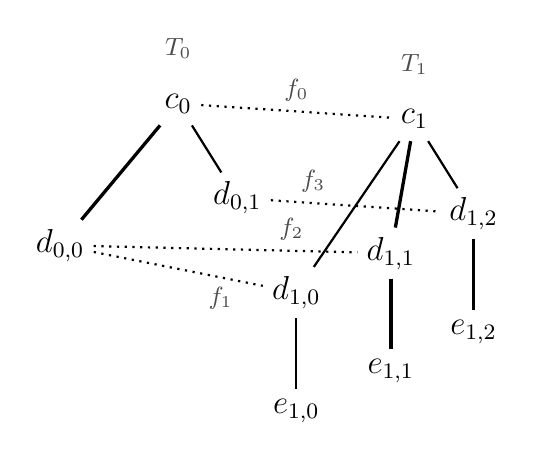
\begin{tikzpicture}[x=1.5cm, y=1cm, thick,
		node/.style={inner sep=3pt, minimum size=1.5em, font=\large{#1}},
		stage/.style={node,opacity=0.7},
		label/.style={node,rotate=-3.5,opacity=0.7},
		edgelabel/.style={opacity=0.7}
]


	\node[node] (c2) at (4, 9.6) {$c_0$};
	\node[node] (c3) at (6, 9.4) {$c_1$};

	\node[node] (d10) at (3, 7.8) {$d_{0,0}$};
	\node[node] (d11) at (4.5, 8.4) {$d_{0,1}$};
	\node[node] (d20) at (5, 7.2) {$d_{1,0}$};
	\node[node] (d21) at (5.8, 7.7) {$d_{1,1}$};
	\node[node] (d22) at (6.5, 8.2) {$d_{1,2}$};

	\node[node] (e00) at (5, 5.7) {$e_{1,0}$};
	\node[node] (e01) at (5.8, 6.2) {$e_{1,1}$};
	\node[node] (e02) at (6.5, 6.7) {$e_{1,2}$};

	\node[stage] (l3) at (4,10.3) {\small $T_0$};
	\node[stage] (l4) at (6,10.1) {\small $T_1$};
	
	\draw[dotted] (c2) -- (c3) node [edgelabel, midway, above] {\small $f_0$};



	% Stage 2
	\draw[very thick] (c2) -- (d10);
	\draw (c2) -- (d11);

	% Stage 3
	\draw (c3) -- (d20);
	\draw[very thick] (c3) -- (d21);
	\draw (c3) -- (d22);
	\draw[dotted] (d10) -- (d20) node [edgelabel, near end, below] {\small $f_1$};;
	\draw[dotted] (d10) -- (d21) node [edgelabel, near end, above] {\small $f_2$};;
	\draw[dotted] (d11) -- (d22) node [edgelabel, near start, above] {\small $f_3$};;

	% Stage 4
	\draw (d20) -- (e00);
	\draw[very thick] (d21) -- (e01);
	\draw (d22) -- (e02);


\end{tikzpicture}
}
\end{center}
\caption{In this example, the refinement tree $R$ whose nodes are $\{f_0, f_1, f_2, f_3\}$ witnesses 
the extension of the stage tree $T_0$ whose nodes are $\{c_0, d_{0,0}, d_{0,1}\}$ 
by the stage tree $T_1$ whose nodes are $\{c_1, d_{1,0}, d_{1,1}, d_{1,2}, e_{1,0}, e_{1,1}, e_{1,2}\}$.
The condition~$c_1$ has three parts, and $f_0$-refines the condition~$c_0$ which has two parts.
The conditions $d_{1,0}$, $d_{1,1}$ and~$d_{1,2}$ have only one part.
The path $c_1 \-- d_{1,1} \-- e_{1,1}$ trough the tree $T_1$ $R$-refines the path $c_0 \-- d_{0,0}$
through the tree $T_0$.}
\end{figure}

At each stage, we will extend the current stage tree to a stage tree of larger depth
and whose conditions force more and more properties. The resulting
sequence of stage trees $T_0 \geq T_1 \geq \dots$ can be seen as a 2-dimensional tree
with the following axes:

\begin{itemize}
	\item The \emph{stage axis} is a temporal dimension.
	Let $c_0 \geq c_1 \geq \dots$ be such that $c_s$ is the root of $T_s$ for each stage~$s$.
	As we saw in the computable non-reducibility case, the parts of this sequence forms
	an infinite, finitely branching tree. Let $P$ be any infinite path through this tree.
	More formally, $P$ is a sequence $\nu_0, \nu_1, \dots$ such that $\nu_{s+1}$ is a part of~$c_{s+1}$
	refining the part~$\nu_s$ in~$c_s$ for each~$s$. Consider now the sequence
	of stage trees~$T_0^{[\nu_0]} \geq T_1^{[\nu_1]} \geq \dots$ The sequence lives at the second iteration level,
	below the path~$P$. Its roots induce another infinite, finitely branching tree, and so on.
	Therefore, at each level, we can define an infinite, finitely branching tree of parts,
	once we have fixed the path $P$ through the tree of parts at the previous level.

	\item The \emph{iteration axis} is a spatial (or vertical) dimension corresponding to the depth.
	The notion of stage tree makes explicit the finite tree obtained when fixing a stage.
	A path through a stage tree corresponds to the choices made at each level, between the different
	parts of a condition. We did not define the notion of acceptable part in this framework.
	Therefore, the choice of the part is delegated to the module, which will have to justify that
	at least one of the parts is extensible.
\end{itemize}

\begin{definition}[Partial path]
A \emph{partial path} $\rho$ through a stage tree $T$ of depth~$n$ is defined inductively as follows:
A partial path through a stage tree $T$ of depth 0 is a part of $T$.
A partial path through a stage tree $T = \tuple{c, h}$ of depth $n+1$ is either a part of $c$,
or a sequence $\nu, \rho$ where $\nu$ is a part of $c$ 
and $\rho$ is a partial path through $h(\nu)$.
A \emph{path} through $T$ is a partial path of length~$n+1$.
\end{definition}

We denote by $P(T)$ and by $PP(T)$ the collection of paths and partial paths through $T$, respectively.
Note that a partial path has length at least 1. The notion of refinement between
partial paths is defined in the natural way. We can also extend the notation
$T^{[\rho]}$ to partial paths $\rho$ through~$T$ with the obvious meaning.
There is also a notion of satisfaction of a stage tree induced by the $\satop$ operator.

\begin{definition}[Stage tree satisfaction]
A set $G_0$ \emph{satisfies} a partial path $\nu_0$ 
through a stage tree $T$ of depth~$0$ 
if $G_0 \in \satop(\nu_0)$.
A tuple of sets $G_0, G_1, \dots, G_k$ \emph{satisfies} a partial path $\nu_0, \dots, \nu_k$ 
through a stage tree $T = \tuple{c,h}$ of depth~$n+1$ if $G_0 \in \satop(\nu_0)$
and $k = 0$, or $G_1, \dots, G_k$ satisfies the partial path $\nu_1, \dots, \nu_k$ through
the stage tree $h(\nu_0)$.
A tuple of sets $G_0, G_1, \dots, G_k$ \emph{satisfies} a stage tree $T$ of depth~$n$
if it satisfies a partial path through $T$.
\end{definition}

Again, if $G_0, \dots, G_k$ satisfies a stage tree of depth~$n$,
then $k \leq n$. The notion of satisfaction induces a forcing relation.
We say that $T$ \emph{forces} some formula $\varphi(D, G)$ below a partial path $\rho = \nu_0, \dots, \nu_k$
(written $T \Vdash_\rho \varphi(U, G)$ if for every tuple of sets $G_0, \dots, G_k$
satisfying $\nu_0, \dots, \nu_k$, $\varphi(\bigoplus_{i < k} G_i, G_k)$ holds.

We now prove a few lemmas stating that we can compose locally the abstract operators
to obtain some global behavior. The first trivial lemma shows how to increase the size of a stage tree.
This is where we use the operator $\iniop$.

\begin{lemma}[Growth lemma]\label{lem:growth-lemma}
For every stage tree $T_0$ of depth $n$ and every~$m$,
there is a stage tree $T_1$ of depth $n+1$ such that $T_1 \uh n = T_0$,
and whose leaves are~$\iniop(m)$.
Moreover, $T_1$ can be computably found uniformly in $T_0$.
\end{lemma}
\begin{proof}
The proof is done inductively on the depth of~$T_0$.
In the base case, $T_0$ is a stage tree of depth 0 and is therefore a condition~$c_0$.
Let $h$ be the function such that~$h(\nu) = \iniop(m)$ for each~$\nu \in \parop(c_0)$.
The tuple~$T_1 = \tuple{c_0, h}$ is a stage tree of depth 1 such that $T_1 \uh 0 = c_0 = T_0$.
It can be computably found uniformly in $T_0$ since $\iniop$ and $\parop$ are computable.
Suppose now that $T_0 = \tuple{c_0, h_0}$ is a stage tree of depth $n+1$. By induction hypothesis,
we can define a function $h_1$ such that for each~$\nu \in \parop(c_0)$, $h_1(\nu)$ is a stage tree of depth $n+1$
and $h_1(\nu) \uh n = h_0(\nu)$. The tuple $T_1 = \tuple{c_0, h_1}$ is a stage tree of depth $n+2$
such that $T_1 \uh n+1 = \tuple{c_0, h_0} = T_0$.
\end{proof}

We will always apply the growth lemma in the case~$m = n+1$. However, the full statement
was necessary to apply the induction hypothesis.
Note that, since $T_1 \uh n = T_0$, we have $T_1 \leq T_0$ as witnessed
by taking the refinement tree of identity functions.
The next lemma states that we can, given some stage tree $T_0$
and some query~$\varphi(D, G)$, obtain another stage tree $T_1 \leq T_0$ in which 
we have decided $\varphi(D, G)$ at every part of every condition in $T_0$.
Its proof is non-trivial since when forcing some property, we may increase the number
of branches of the stage tree. We need therefore to define some elaborate decreasing property
to prove termination of the procedure. The query lemma is assumed yet 
and will be proven in subsection~\ref{subsect:queries-detailed}.

\begin{lemma}[Query lemma]\label{lem:query-lemma}
Let $T_0$ be a stage tree of depth~$n$
and ~$q : PP(T) \to \queryop[D,G]$ be a computable function.
There is a stage tree $T_1 \leq T_0$ of depth $n$
such that every partial path $\xi$ through $T_1$ refines a partial path $\rho$ through $T_0$
for which $T_1 \Vdash_\xi q(\rho)$ or $T_1 \Vdash_\xi \neg q(\rho)$,
Moreover, $T_1$ and the function of answers $a : PP(T_1) \to \ansop[D,G]$ can be $\Delta^0_2$-found
uniformly from $T_0$.
\end{lemma}

The following domination lemma is a specialization of the query lemma
by considering queries about termination of programs.

\begin{lemma}[Domination lemma]\label{lem:domination-lemma}
For every stage tree $T_0$ of depth~$n$, there is
a stage of tree $T_1 \leq T_0$ of depth~$n$ and a finite set $U \subset \omega$ such that
for every tuple~$G_0, \dots, G_n$ satisfying $T_1$ and every $e, x, i \leq n$,
$\Phi_e^{G_0 \oplus \dots \oplus G_i}(x) \in U$ whenever $\Phi_e^{G_0 \oplus \dots \oplus G_i}(x)$ halts.
Moreover, $T_1$ and $U$ can be $\Delta^0_2$-found uniformly from $T_0$.
\end{lemma}
\begin{proof}
Apply successively the query lemma with $q(\xi) = (\exists s,m)\Phi_{e,s}^{D \oplus G}(x) \downarrow = m$
for each~$e, x \leq n$, in order to obtain the tree $T_1$ together with an upper bound $k$ to the answers to $q(\rho)$.
We claim that the set $U = [0, k]$ satisfies the desired property.
Let~$G_0, \dots, G_n$ be a tuple satisfying $T_1$, and let~$e, x, i < n$
be such that $\Phi_e^{G_0 \oplus \dots \oplus G_i}(x) \downarrow$.
By definition of satisfaction, there is some partial path $\rho$ through $T_1$
such that $G_0, \dots, G_i$ satisfies $\rho$. By the query lemma,
$T_1 \Vdash_\rho (\exists s,m)\Phi_{e,s}^{D \oplus G}(x) \downarrow = m$
or $T_1 \Vdash_\rho \neg (\exists s,m)\Phi_{e,s}^{D \oplus G}(x) \downarrow = m$.
Since $\Phi_e^{G_0 \oplus \dots \oplus G_i}(x) \downarrow$, the former holds,
and $k$ is greater than the answer to the query, so is greater than $m$.
Uniformity is inherited from the query lemma.
\end{proof}


We construct an infinite $\Delta^0_2$ sequence of finite trees of conditions $T_0 \geq T_1 \geq \dots$ as follows:
At stage 0, we start with a stage tree $T_0$ of depth 0 defined by $\iniop(0)$.
At each stage $s > 0$, assuming we have defined a stage tree $T_{s-1}$ of depth~$s-1$, act as follows:
\begin{itemize}
	\item[(S1)] \emph{Growth}: Apply the growth lemma to obtain a stage tree $T^1_s \leq T_{s-1}$
	of depth $s$.
	Intuitively, this step adds a new iteration and therefore ensures that the construction will have eventually
	infinitely many levels of iteration.

	\item[(S2)] \emph{Progress}: Apply to $T^1_s$ the query lemma with $q = \progop$ to obtain a stage
	tree $T^2_s \leq T^1_s$ such that the progress function is forced at each partial path.
	This step ensures that for every tuple $G_0, G_1, \dots$ such that $G_0, \dots, G_k$
	satisfies each $T_s$, $s \geq k$, the progress query will have been decided
	on $G_i$ infinitely many times.

	\item[(S3)] \emph{Domination}: Apply to $T^2_s$ the domination lemma to obtain
	a stage tree $T_s \leq T^2_s$ and a finite set $U$ such that for every tuple $G_0, \dots, G_s$
	satisfying $T_s$ and every $e, x, i \leq s$, if $\Phi_e^{G_0 \oplus \dots \oplus G_i}(x)$ halts,
	then its value will be in $U$. Since the whole construction is $\Delta^0_2$
	and we uniformly find such a set $U$, this step enables us to define a $\Delta^0_2$
	function which will dominate every function in the Turing ideal.
\end{itemize}

\subsection{Queries}\label{subsect:queries-detailed}

In this section, we develop the tools necessary to prove the query lemma (Lemma~\ref{lem:query-lemma}).
Given some stage tree $T_0$ and some query function $q : PP(T) \to \queryop[D, G]$, the query lemma
states that we can find a stage tree $T_1$ extending $T_0$ and which forces either $q(\rho)$
or its negation on each partial path through $T_1$ refining the partial $\rho$ through $T_0$.
The stage tree $T_0$ is finite and has therefore finitely many partial paths.
The naive algorithm would consist of taking an arbitrary partial path $\rho$ through $T_0$,
then decide $q(\rho)$ thanks to the process illustrated in Figure~\ref{fig:boxing-sequence} and extend $T_0$
into a stage tree $T_1$ which forces $q(\rho)$ or its negation on every path refining $\rho$.
One may expect to obtain the query lemma by iterating this process finitely many times.

The termination of the algorithm depends on the shape of the extension $T_1$ obtained
after deciding $q(\rho)$. We need to ensure that we made some progress so that we will
have covered all paths at some point. Let us look more closely at the construction of the extension $T_1$.
Given some query $\varphi(D, G)$ and some part~$\nu$, we call the $\unboxop(\nu, \varphi)$ operator to obtain another
query $\psi(D)$ getting rid of the forcing variable $G$. Using $\emptyset'$, we obtain an answer $a$
to the formula $\varphi(\emptyset)$ and then call $\unboxop(\nu, a)$ to obtain some extension 
forking only~$\nu$, and forcing either $\varphi(D,G)$ or its negation on every part refining~$\nu$.
This extension may therefore increase the number of parts, but ensures some progress on each of the forked parts.

If $T_0$ is a stage tree of depth 0, the termination of the process is clear.
Indeed, $T_0$ is a condition~$c_0$ and the partial paths through $T_0$ are simply the parts of $c_0$.
We end up with a stage tree $T_1$ of depth 0 corresponding to some condition~$c_1$,
on which we have decided $\varphi(D,G)$ for every part of $c_1$ refining some part~$\nu$ of~$c_0$.
Since we have not forked any other part than $\nu$, the number of undecided parts strictly decreases.
A condition has finitely many parts, so the process terminates after at most $|\parop(c_0)|$
steps.

The progress becomes much less clear if $T_0$ is a stage tree of depth 1.
When trying to decide some query on some path $\nu_0,\nu_1$ through $T_0$, we need to extend
both the root, and the conditions below each part~$\mu$ refining $\nu_0$.
The overall number of undecided paths may increase, and therefore a simple cardinality argument
is not enough to deduce termination.
Note that this algorithm has some common flavor with the \emph{hydra game}
introduced by Kirby and Paris~\cite{Kirby1982Accessible} and whose termination
is not provable in Peano arithmetic. Thankfully, our problem is much simpler
and its termination can be proven by elementary means.

\begin{figure}[htbp]
\begin{center}
\scalebox{0.9}{
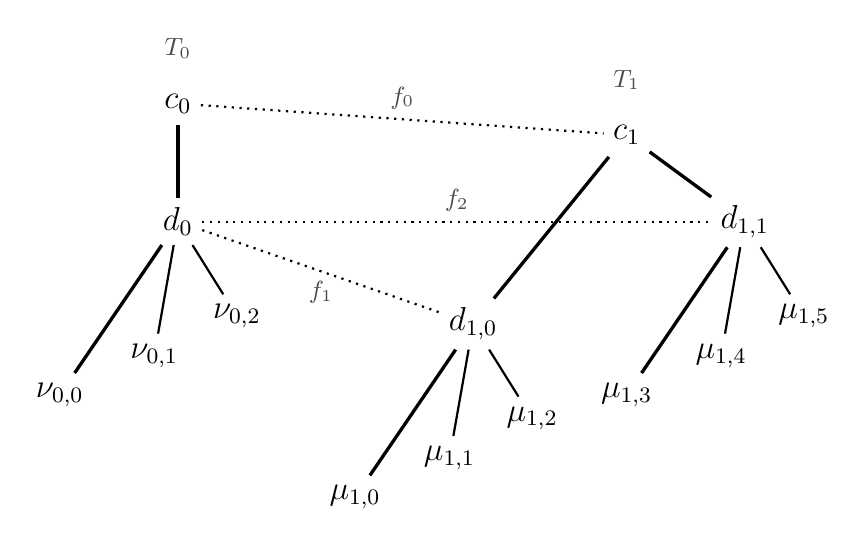
\begin{tikzpicture}[x=1.5cm, y=1cm, thick,
		node/.style={inner sep=3pt, minimum size=1.5em, font=\large{#1}},
		stage/.style={node,opacity=0.7},
		label/.style={node,rotate=-3.5,opacity=0.7},
		edgelabel/.style={opacity=0.7}
]


	% Stage 0
	\node[node] (c0) at (4, 9.8) {$c_0$};
	\node[node] (d0) at (4, 8.3) {$d_0$};
	\node[node] (e00) at (3, 6.1) {$\nu_{0,0}$};
	\node[node] (e01) at (3.8, 6.6) {$\nu_{0,1}$};
	\node[node] (e02) at (4.5, 7.1) {$\nu_{0,2}$};


	% Stage 1
	\node[node] (c1) at (7.8, 9.4) {$c_1$};
	\node[node] (d10) at (6.5, 7) {$d_{1,0}$};
	\node[node] (d11) at (8.8, 8.3) {$d_{1,1}$};

	\node[node] (e10) at (5.5, 4.8) {$\mu_{1,0}$};
	\node[node] (e11) at (6.3, 5.3) {$\mu_{1,1}$};
	\node[node] (e12) at (7, 5.8) {$\mu_{1,2}$};

	\node[node] (e13) at (7.8, 6.1) {$\mu_{1,3}$};
	\node[node] (e14) at (8.6, 6.6) {$\mu_{1,4}$};
	\node[node] (e15) at (9.3, 7.1) {$\mu_{1,5}$};


	\node[stage] (l3) at (4,10.5) {\small $T_0$};
	\node[stage] (l4) at (7.8,10.1) {\small $T_1$};
	
	\draw[dotted] (c0) -- (c1) node [edgelabel, midway, above] {\small $f_0$};



	% Stage 0
	\draw[very thick] (c0) -- (d0);
	\draw[very thick] (d0) -- (e00);
	\draw (d0) -- (e01);
	\draw (d0) -- (e02);



	% Stage 1
	\draw[very thick] (c1) -- (d10);
	\draw[very thick] (c1) -- (d11);

	\draw[very thick] (d10) -- (e10);
	\draw (d10) -- (e11);
	\draw (d10) -- (e12);

	\draw[very thick] (d11) -- (e13);
	\draw (d11) -- (e14);
	\draw (d11) -- (e15);

	\draw[dotted] (d0) -- (d10) node [edgelabel, midway, below] {\small $f_1$};
	\draw[dotted] (d0) -- (d11) node [edgelabel, midway, above] {\small $f_2$};
	%\draw[dotted] (e00) -- (e10);
	%\draw[dotted] (e01) -- (e11);
	%\draw[dotted] (e02) -- (e12);
	%\draw[dotted] (e00) -- (e13);
	%\draw[dotted] (e01) -- (e14);
	%\draw[dotted] (e02) -- (e15);

\end{tikzpicture}
}
\end{center}
\caption{In this example, we start with a stage tree $T_0$ of depth 1 and want to decide some query $\varphi(D,U)$
for each of its three paths. We choose one path $\rho = c_0 \-- d_0 \-- \nu_{0,0}$,
call $\boxop(\nu_{0,0}, \varphi)$ to obtain a query $\psi(D)$, then call $\boxop(\lambda, \psi)$,
where $\lambda$ is the unique part of~$c_0$.
We obtain a query $\phi(D)$, $\emptyset'$-compute some answer $a$ to $\phi(\emptyset)$
and call $\unboxop(\lambda, a)$ to obtain some extension $c_1$ of $c_0$ and some answering function $b : \parop(c_1) \to \ansop[D,G]$. This extension forks the part $\lambda$ into two parts. Below each part $\lambda_i$ in $c_1$, we call $\unboxop(\lambda_i, b(\lambda_i))$
to obtain an extension of $d_{1,i}$ forcing $\varphi(D,G)$ below the parts refining $\nu_{0,0}$.}
\label{fig:refinement-query-progress}
\end{figure}

In Figure~\ref{fig:refinement-query-progress}, we give an example of one step in the decision process,
starting with a stage tree $T_0$ of depth $1$ with three undecided paths, and ending up with
some stage tree $T_1$ having four undecided paths ($c_1 \-- d_{1,0} \-- \mu_{1,1}$, $c_1 \-- d_{1,0} \-- \mu_{1,2}$,
$c_1 \-- d_{1,0} \-- \mu_{1,1}$ and $c_1 \-- d_{1,0} \-- \mu_{1,2}$).
Thankfully, the $\unboxop$ operator forks only the part on which it answers the query. Therefore,
at the next step, we will be able to consider only one of the parts of $c_1$ at a time.
The induced subtree has two undecided paths, so there is also some progress.

We now define some relation $\sqsubset$ between two stage trees $T_0$ and $T_1$ of depth $n$.
It describes the relation between the stage tree $T_0$ and the extension $T_1$ obtained after
applying one step of the query algorithm. More precisely, $T_2 \sqsubset T_0$
if $T_2$ is the subtree of $T_1$ on which we have removed every decided paths.

\begin{definition}
Given two stages trees $T_1 \leq T_0$ of depth~$n$,
we define the relations $T_1 \sqsubseteq T_0$ and $T_1 \sqsubset T_0$ by mutual induction as follows.
If $T_0$ and $T_1$ are conditions and $T_1 \leq_f T_0$, then 
$T_1 \sqsubseteq T_0$ if $f$ does not fork any part of~$T_0$. 
If moreover $f$ is not surjective, then $T_1 \sqsubset T_0$.
If $T_1 = \tuple{c_1, h_1}$, $T_0 = \tuple{c_0, h_0}$ and $c_1 \leq_f c_0$,
then $T_1 \sqsubseteq T_0$ if for every part $\nu$ of $c_1$,
if $f$ forks part~$f(\nu)$ of $c_0$ then $h_1(\nu) \sqsubset h_0(f(\nu))$,
otherwise $h_1(\nu) \sqsubseteq h_0(f(\nu))$. If moreover there is some part~$\mu$ of $c_0$
such that $h_1(\nu) \sqsubset h_0(\mu)$ for every part~$\nu$ of $c_1$ refining $\mu$,
then $T_1 \sqsubset T_0$.
\end{definition}

One easily proves by mutual induction over the depth of the trees the following facts:
\begin{itemize}
	\item[(i)] Both~$\sqsubset$ and~$\sqsubseteq$ are transitive
	\item[(ii)] If~$T_1 \sqsubset T_0$ then~$T_1 \sqsubseteq T_0$
	\item[(iii)] If~$T_2 \sqsubseteq T_1$ and~$T_1 \sqsubset T_0$ then~$T_2 \sqsubset T_0$
	\item[(iv)] If~$T_2 \sqsubset T_1$ and~$T_1 \sqsubseteq T_0$ then~$T_2 \sqsubset T_0$
\end{itemize}
Assuming that $\sqsubset$ truly represents the relation between a stage tree
and its extension after one step of query, the following lemma
can be understood as stating that the naive algorithm used in the proof of the query lemma terminates.

\begin{lemma}\label{lem:sq-well-founded}
The relation $T_1 \sqsubset T_0$ is well-founded.
\end{lemma}
\begin{proof}
By induction over the depth of the stage trees.
Suppose that $T_0 \sqsupset T_1 \sqsupset \dots$ is an infinite
decreasing sequence of stage trees of depth 0.
In particular, the $T$'s are conditions and $T_0 \geq_{f_0} T_1 \geq_{f_1} \dots$
for some functions $f_i$ which are injective, but not surjective. Therefore
the number of parts strictly decreases in $\omega$, contradiction.

Suppose now that $T_0 \sqsupset T_1 \sqsupset \dots$ is an infinite
decreasing sequence of stage trees of depth $n+1$,
where $T_i = \tuple{c_i, h_i}$ and $c_i \geq_{f_i} c_{i+1}$.
Let $S$ be the set of parts~$\nu$ in some~$c_i$
which will fork at a later $c_j$. This $S$ induces a finitely branching tree.
If $S$ is finite, then there is some~$j$ such that no part of~$c_k$ will ever fork for every~$k \geq j$.
By the infinite pigeonhole principle, there we can construct an infinite, decreasing sequence
of trees of depth $n$, contradicting our induction hypothesis. So suppose that $S$ is infinite.
By König's lemma, there is an infinite sequence of parts, the later refining the former,
such that they fork. Each time a conditions fork, the subtree is strictly decreasing, so we can
define an infinite decreasing sequence of stage trees of depth $n$, again contradicting our induction hypothesis.
\end{proof}

Given some stage tree $T_1$ of depth $i < n$, a \emph{completion of $T_1$ to $n$}
is a stage tree $T_2$ of depth $n$ such that $T_1 \uh i = T_0$.
If $T_1 \leq T_0 \uh i$ for some stage tree $T_0$ of depth $n$,
$T_0$ induces a completion $T_2$ of $T_1$ to $n$ by setting $T_2^{[\xi]} = T_0^{[\rho]}$
for every path $\xi$ through $T_1$ refining some path $\rho$ through $T_0 \uh i$.
One easily checks that $T_2 \leq T_0$.
Such a stage tree is called the \emph{trivial completion of $T_1$ by~$T_0$}.
The following technical lemma will be useful for applying 
the induction hypothesis in Lemma~\ref{lem:sq-one-step-forcing}.

\begin{lemma}\label{lem:sq-concatenation}
Let $T_0, T_1$ be two stage trees of depth $n+1$ and $T_2$ be a stage tree of depth $n$ 
and $S_0$ be a set of paths through $T_0 \uh n$ such that
\begin{itemize}
	\item[(i)] $T_2 \sqsubseteq T_0 \uh n$, $P(T_2) \subseteq P(T_1 \uh n)$ and $T_1 \leq T_0$
	\item[(ii)] $S_0$ is the set of paths through $T_0 \uh n$ refined by some path through $T_2$.
	\item[(iii)] For every path $\xi \in P(T_2)$, $T_1^{[\xi]} \sqsubseteq T_0^{[\rho]}$ where $\xi$ refines the path $\rho \in S_0$	
	\item[(iv)] For every path $\xi \in P(T_1 \uh n) \setminus P(T_2)$, $\xi$ refines some path $\rho \in P(T_0 \uh n) \setminus S_0$
	and $T_1^{[\xi]} \sqsubset T_0^{[\rho]}$
\end{itemize}
Then $T_1 \sqsubseteq T_0$. Moreover, if $T_2 \sqsubset T_0 \uh n$ then $T_1 \sqsubset T_0$.
\end{lemma}
\begin{proof}
By induction over $n$. In the base case, $T_0 \uh n$, $T_1 \uh n$ and $T_2$
are conditions $c_0$, $c_1$ and $c_2$ such that $c_2 \leq_f c_0$ and $c_1 \leq_g c_0$ for some refinement functions $f$ and $g$.
We easily have $T_1 \sqsubseteq T_0$ since $T_1^{[\mu]} \sqsubseteq T_0^{[g(\nu)]}$ for every
part $\mu$ of $c_2$ (and therefore of~$c_1$),
and since $T_1^{[\mu]} \sqsubset T_0^{[g(\nu)]}$ whenever $\mu$ is a part of~$c_1$ which is not a part of~$c_2$. 
By $c_2 \sqsubseteq c_0$, the only places where a fork can happen is when $\mu$ is not in $c_2$.

We now want to prove that $T_1 \sqsubset T_0$ whenever~$c_2 \sqsubset c_0$.
Since $c_2 \sqsubset c_0$, $f$ is injective, but not surjective. We need to prove that there is some part~$\nu$ of $T_1$ such that $T_1^{[\nu]} \sqsubset T_0^{[g(\nu)]}$. We have two cases. In the first case, $f$ and $g$ have the same domain. In this case $f = g$ and since $f$ is not surjective, 
there is some part of~$c_0$ witnessing the strictness of $T_1 \sqsubset T_0$.
In the second case, there is some part~$\nu$ in $c_1$ but not $c_2$. By (iv), $g(\nu) \not \in S_1$. The part~$g(\nu)$ of $c_0$ witnesses the stricteness of $T_1 \sqsubset T_0$.

In the induction case, $T_0 \uh n = \tuple{c_0, h_0}$, $T_1 \uh n = \tuple{c_1, h_1}$ and $T_2 = \tuple{c_2, h_2}$
such that $c_2 \leq_f c_0$ and $c_1 \leq_g c_0$ for some refinement functions $f$ and $g$.
For every part~$\nu$ in $c_1$, we have two cases:
In the first case, $\nu$ is not in $c_2$. By (iv), any path $\xi$ through $h_1(\nu)$
refines some path $\rho$ in $h_0(g(\nu))$ such that $h_1(\nu)^{[\xi]} \sqsubset h_0(g(\nu))^{[\rho]}$.
By the induction hypothesis applied to $h_0(\nu)$, $h_1(\nu)$ and the empty tree, $h_1(\nu) \sqsubset h_0(g(\nu))$.
In the second case, $\nu$ is also in $c_2$. By the induction hypothesis applied to $h_0(\nu)$, $h_1(\nu)$
and $h_2(\nu)$, $h_1(\nu) \sqsubseteq h_0(g(\nu))$.
We again easily have $T_1 \sqsubseteq T_0$ since $h_1(\nu) \sqsubseteq h_0(g(\nu))$ for every part~$\nu$ in $c_1$
and since whenever $g$ forks some part~$\mu$ of~$c_0$, either the parts $\nu$ of $c_1$ refining $\mu$
are all in $c_2$ in which case $h_2(\nu) \sqsubset h_0(\mu) \uh n$ by the definition of the partial order and then we have $h_1(\nu) \sqsubset h_0(\mu)$, or none of the parts $\nu$ of $c_1$ refining $\mu$ are in $c_2$,
in which case we have $h_1(\nu) \sqsubset h_0(\mu)$.
By the same case analysis as in the base case, we deduce that $T_1 \sqsubset T_0$
if moreover $T_2 \sqsubset T_0 \uh n$.
\end{proof}

\begin{definition}[Stage tree substration]
Given a stage tree $T$ of depth $n$ and a set $S$ of paths through $T$,
we define $T - S$ inductively as follows:
If $T$ is a stage tree of depth 0, then $S$ is a set of parts of $T$
and $T - S$ is the condition whose parts are $\parop(T) \setminus S$.
If $T = \tuple{c, h}$ is a stage tree of depth $n+1$, then $S$ is a set of paths of the form
$\nu\rho$ where $\nu$ is a part of $c$ and $\rho$ is a path through $h(\nu)$.
For each part~$\nu$, let $S_\nu = \{ \rho : \nu\rho \in S\}$.
The stage tree $T - S$ is defined by $\tuple{c, h_1}$ where $h_1(\nu) = h(\nu) - S_\nu$
for each part $\nu$ of $c$.
\end{definition}

Intuitively, $T - S$ is the maximal subtree of $T$ such that
$P(T - S) = P(T) \setminus S$. Beware, even if we may remove every part of a condition,
we do not remove the condition from the tree.
The following lemma uses the well-founded partial order
defined previously to show that we can make some progress
in deciding the queries. In what follows, the set~$T_0$ can be thought of as
the stage tree we obtain after having applied finitely many steps
of query and $S_0$ are the paths through the tree~$T_0$ for which we have already
decided the query~$\varphi(D, G)$. The lemma describes the relation
between the state~$(T_1, S_1)$ obtained from~$(T_0, S_0)$ after having applied one more step.

\begin{lemma}\label{lem:sq-one-step-forcing}
Let $T_0$ be a stage tree of depth $n$, $S_0$ be a set of paths through $T_0$ and let~$\varphi(D,G)$ be a query.
For every path $\rho \not \in S_0$ through $T_0$, there exists a stage tree $T_1 \leq T_0$ of depth $n$
and a set $S_1$ of paths through $T_1$ such that
\begin{itemize}
	\item[(i)] $T_1 \Vdash_\xi \varphi(D,G)$ or $T_1 \Vdash_\xi \neg \varphi(D, G)$ for every
	path $\xi$ through $T_1$ refining $\rho$.
	\item[(ii)] $T_1 - S_1 \sqsubset T_0 - S_0$
	\item[(iii)] Every path in $S_1$ refines either a path in $S_0$ or $\rho$.
\end{itemize}
Moreover, $T_1$ and the function of answers $a : P(T_1) \to \ansop[D,G]$
can be $\emptyset'$-effectively computed uniformly in $T_1$ and $\varphi(D,G)$.
\end{lemma}
\begin{proof}
By induction over $n$.
If $T_0$ is a stage tree of depth 0, then it is a condition $c_0$
and the paths through $T_0$ are the parts of~$c_0$. Let~$\nu$ be such a part.
Let~$\psi(D)$ be the query $\boxop(\nu, \varphi)$.
We can $\emptyset'$-compute an answer $a_0$ to $\psi(\emptyset)$.
Let~$\tuple{c_1,f,a} = \unboxop(\nu, a_0)$ be such that $c_1 \leq_f c_0$,
$f$ forks only part~$\nu$ of $c_0$ and for every part~$\mu$ of $c_1$ such that $f(\mu) = \nu$,
$c_1 \Vdash_\mu \varphi(D, G)$ or $c_1 \Vdash_\mu \neg \varphi(D, G)$ and $a(\mu)$
answers $\varphi(D,G)$ accordingly. Take $S_1 = \{ \mu : f(\mu) = \nu \vee f(\mu) \in S_0\}$.
The property (i) holds by definition of $c_1$ and (iii) holds by definition of $S_1$.
Since the only forked part is $\nu$ and no part of~$c_1 - S_1$ refines $\nu$,
$c_1 - S_1 \sqsubset c_0 - S_0$, so the property (ii) also holds. This completes the base case.

Suppose now that $T_0$ is a stage tree of depth~$n+1$.
The paths through $T_0$ are of the form $\rho\nu$
where $\rho$ is a path through $T_0 \uh n$ and $\nu$ is a part of the root of $T_0^{[\rho]}$.
Fix any such path. Let~$\psi(D)$ be the query $\boxop(\nu, \varphi)$
and let $\phi(D, G)$ be the formula $\psi(D \oplus G)$.
By induction hypothesis on $T_0 \uh n$, there is a stage tree $T_2 \leq T_0 \uh n$
and a set $S_2$ such that
\begin{itemize}
	\item[(i)] $T_2 \Vdash_\xi \phi$ or $T_2 \Vdash_\xi \neg \phi$ for every
path $\xi$ through $T_2$ refining $\rho$
	\item[(ii)] $T_2 - S_2 \sqsubset T_0 \uh n - S_0 \uh n$
	\item[(iii)] Every path in $S_2$ refines either a path in $S_0 \uh n$
	or $\rho$.
\end{itemize}
Moreover, still by induction hypothesis, we have a function $a : P(T_2) \to \ansop[D, G]$
answering the queries. We define a completion of $T_2$ into a stage tree $T_1$
of depth $n+1$ as follows: For each path $\xi$ through $T_2$ refining $\rho$,
let $T_1^{[\xi]}$ be the condition~$c_\xi$ such that $\tuple{c_\xi, f_\xi, a_\xi} = \unboxop(\nu, a(\xi))$.
For each path $\xi$ through $T_2$ which refines some path $\tau$ through $T_0$ different from $\rho$, let $T_1^{[\xi]} = T_0^{[\tau]}$.
By construction, $T_1 \leq T_0$ since $c_\xi$ $f_\xi$-refines $T_0^{[\rho]}$ whenever $\xi$ refines $\rho$
and since any condition refines itself. Let $S_1$ be the collection of paths $\xi\mu$
through $T_1$ such that $\xi \in S_2$ and either $\xi$ refines $\rho$ and $f_\xi(\mu) = \nu$, or $\xi\mu$
refines a path in $S_0$. Since $(T_0 \uh n - S_0 \uh n) \sqsubseteq (T_0 - S_0) \uh n$,
we have $T_2 - S_2 \sqsubset (T_0 - S_0) \uh n$. We can therefore apply Lemma~\ref{lem:sq-concatenation} to $T_0 - S_0$, $T_1 - S_1$, and $T_2 - S_2$, to obtain $T_1 - S_1 \sqsubset T_0 - S_0$.
Define the answer function $b : P(T_1) \to \ansop[D, G]$ by $b(\xi\mu) = a_\xi(\mu)$
for each path $\xi$ through $T_2$ refining $\rho$. This function $b$ is found $\emptyset'$-effectively
since the $\unboxop$ operator is computable.
\end{proof}

The following lemma simply iterates Lemma~\ref{lem:sq-one-step-forcing}
and uses the well-foundedness of the relation $\sqsubset$ to deduce
that we can find some extension on which the queries are decided for every path.

\begin{lemma}\label{lem:sq-one-level-forcing}
Let $T_0$ be a stage tree of depth $n$ and let~$q : P(T_0) \to \queryop[D,G]$ be a function.
There is a stage tree $T_1 \leq T_0$ of depth $n$ such that
$T_1 \Vdash_\xi q(\rho)$ or $T_1 \Vdash_\xi \neg q(\rho)$ for every
path $\xi$ through $T_1$ refining some path $\rho$ through $T_0$.
Moreover, $T_1$ and the function of answers $a : P(T_1) \to \ansop[D,G]$
can be $\emptyset'$-effectively computed uniformly in $T_1$ and $q$.
\end{lemma}
\begin{proof}
Using Lemma~\ref{lem:sq-one-step-forcing}, 
define a sequence of tuples $\tuple{T_0, S_0, \rho_0, \tau_0}, \tuple{T_1, S_1, \rho_1, \tau_1}, \dots$
starting with $T_0$, $S_0 = \emptyset$, $\rho_0 = \tau_0 \in P(T_0)$
and such that for each~$i$
\begin{itemize}
	\item[(i)] $T_{i+1} \leq T_i$ is a stage tree of depth $n$, $S_i$ is a set of paths through $T_i$
	\item[(ii)] $\rho_i$ is a path through $T_i - S_i$ refining the path $\tau_i$ through $T_0$.
	\item[(iii)] $T_{i+1} \Vdash_\xi q(\tau_i)$ or $T_{i+1} \Vdash_\xi \neg q(\tau_i)$ for every
	path $\xi$ through $T_{i+1}$ refining $\rho_i$
	\item[(iv)] $T_{i+1} - S_{i+1} \sqsubset T_i - S_i$
	\item[(v)] Every path in $S_{i+1}$ refines either a path in $S_i$ or $\rho_i$.
\end{itemize}
By Lemma~\ref{lem:sq-well-founded}, the relation $\sqsubset$ is well-founded, so the sequence has to be finite by (iv). 
Let $k$ be the maximal index of the sequence.
By maximality of $k$ and by Lemma~\ref{lem:sq-one-step-forcing}, $P(T_k) - S_k = \emptyset$.
Therefore, $P(T_k) = S_k$. Since $S_0 = \emptyset$ and by (v), we can prove by induction over $k$ that
for every path $\xi$ through $T_k$, there is some stage $i < k$ such that $\xi$ refines $\rho_i$.
Thus, by (iii) and by stability of the forcing relation under refinement, $T_k \Vdash_\xi q(\tau_i)$ or $T_k \Vdash_\xi \neg q(\tau_i)$.
Therefore $T_k$ satisfies the statement of the lemma.
The uniformity is inherited from the uniformity of Lemma~\ref{lem:sq-one-step-forcing}.
\end{proof}

Last, we prove the query lemma by iterating the previous lemma at every depth of the stage
tree, to decide the queries on the partial paths.

\begin{proof}[Proof of the query lemma]
Let $T_0$ be a stage tree of depth $n$ and $q : PP(T_0) \to \queryop[U,G]$ be a function.
Using Lemma~\ref{lem:sq-one-level-forcing},
define a decreasing sequence of stage trees $T_0 \geq \dots \geq T_n$  of depth $n$
such that for each~$i < n$, 
\begin{itemize}
	\item[(i)] $T_{i+1}$ is the trivial completion of $T_{i+1} \uh i+1$ by $T_i$.
	\item[(ii)] $T_{i+1} \Vdash_\xi q(\tau)$ or $T_{i+1} \Vdash_\xi \neg q(\tau)$ for every
	path $\xi$ through $T_{i+1} \uh i+1$ refining some path $\tau$ through $T_0 \uh i+1$.
\end{itemize}
To do this, at stage $i < n$, apply Lemma~\ref{lem:sq-one-level-forcing} to $T_i$ with the query function $r : PP(T_i) \to \queryop[U,G]$
defined by $r(\rho) = q(\tau)$ for each path $\rho$ through $T_i \uh i+1$ refining some path $\tau$ through $T_0 \uh i+1$.
Since the forcing relation is stable by refinement, the stage tree $T_n$ satisfies the statement of the query lemma.
The uniformity is again inherited from the uniformity of Lemma~\ref{lem:sq-one-level-forcing}.
\end{proof}

This completes the presentation of the framework. We will now define a module for the Erd\H{o}s-Moser
theorem. In section~\ref{sect:separating-amt-combined}, we will see how to compose modules to obtain stronger separations.


